% gt4ai.tex
% Section 4: Game Theory for Strategic AI

\section{Learning as a Strategic Actor}
\label{sec:gt4ai}

Until now, whatever we tested a learned object against did not change: a
fixed game, a fixed dataset, a fixed set of bidders. It did not react to the object
being judged. In this section it does. An agent's opponents adjust to how it plays; a
market moves once a pricing rule starts running. And in every case we are the ones who pick what the object faces: the opponents it is scored
against, the counterpart it is trained against, the market it is released
into. That choice is made before any result arrives, and it sets the limit on what the result can mean.

Four objects have to be kept apart in what follows. The payoffs may be
\emph{externally assigned}, as when we declare that winning a StarCraft match is
what counts, or they may be \emph{inferred preferences}, recovered from an agent's
own choices rather than set by us. The interaction may be a \emph{designed training
game}, built to shape a policy under an oversight objective, or a \emph{deployed
institution}, which no single participant owns. The first pair fixes what a score
can mean; the second fixes whose objective the game answers to.
Section~\ref{sec:gt4ai:evaluation} works with assigned payoffs and turns to
inferred preferences only at its end, Section~\ref{sec:gt4ai:training} takes up
designed training games, and Section~\ref{sec:gt4ai:governance} takes up deployed
institutions.

The three subsections follow that choice from the claim question to the goal question.
Section~\ref{sec:gt4ai:evaluation} stays with the claim question. An agent's score is only its record against a chosen set of opponents. A
StarCraft agent that beats one set can be beaten by another set built to
exploit it, and that second set can be built on purpose. Section~\ref{sec:gt4ai:training} turns to the goal question, where the game is
designed rather than given. Two debaters arguing before a judge, or a reward model
trained on human comparisons of answer pairs, are only as good as the match between
the designed game and the real oversight goal behind it. Section~\ref{sec:gt4ai:governance}
extends the goal question to deployment. A pricing algorithm changes the very market that
is meant to judge it, and someone must then decide which outcomes count, and whose.

\subsection{Strategic Evaluation against Opponent Populations}
\label{sec:gt4ai:evaluation}

Rock-paper-scissors has no best move: rock beats scissors, scissors beats paper, and
paper beats rock, so the right choice depends entirely on the opponent. Evaluating a
learned agent meets the same problem on a larger scale. As with the StarCraft agent
above, competence is not one number but a record against a chosen set of opponents.
That set can be fixed in advance (every agent facing the same opponents), or
it can adapt, with new opponents added in response to how the agent plays. Either way the
evaluator plays the agent in fresh matches, but must treat a finite list as a substitute for every opponent it might face.

Two questions must not be confused. The first is how well the agent plays a game
whose payoffs \emph{we} set. In StarCraft, winning is the payoff we assign, so the
score just measures play against the chosen opponents. The second question asks what
the agent itself \emph{wants}: whether its choices reveal a utility of its own, such
as a taste for cooperation or an aversion to risk. This second reading is far more
demanding, because the choices must be consistent enough to identify such a utility at all, a requirement that never
arises when we set the payoffs ourselves. Almost all
of this section takes the first view; only at the end, under preference
interpretation, do we turn to the second. Table~\ref{tab:evaluation_methods} lays out
the approaches this section covers and the coverage or validity limit each one carries.

\begin{table}[pos=t]
\centering
\caption{Approaches for evaluating a learned strategic actor, and the coverage or
validity limit each one carries. (Section~\ref{sec:gt4ai:evaluation})}
\label{tab:evaluation_methods}
\footnotesize
\setlength{\tabcolsep}{3.5pt}
\renewcommand{\arraystretch}{1.25}

\begin{tabularx}{\textwidth}{
    >{\raggedright\arraybackslash}p{0.17\textwidth}
    >{\raggedright\arraybackslash}p{0.22\textwidth}
    Y
    Y
}
\toprule
\textbf{Evaluation approach}
& \textbf{Representative methods}
& \textbf{What it measures}
& \textbf{Coverage or validity limit}
\\
\midrule

Empirical game / win-rate table
& Empirical-game analysis~\citep{Wellman2006}; benchmark study~\citep{Balduzzi2018}
& The strength of a policy against a chosen set of opponents
& Only the opponents on the list; a crowded list reweights the average
\\

\addlinespace

Restricted exploitability, with adaptive expansion
& NashConv over a searched class; PSRO expansion~\citep{Lanctot2017}
& The most the best counter actually built could gain
& Only the counters the search produced; an untried one can still exist
\\

\addlinespace

Ranking under non-transitivity
& Nash averaging~\citep{Balduzzi2018}, $\alpha$-Rank~\citep{Omidshafiei2019},
open-ended learning~\citep{Balduzzi2019Open}
& A ranking that keeps cycles rather than a single strength axis
& Relative to the chosen population; adding a strategically important policy can
shift it
\\

\addlinespace

Adversarial robustness
& Bounded attack~\citep{Madry2018}, red teaming~\citep{Perez2022}, certified
radius~\citep{CohenRosenfeldKolter2019}
& The worst outcome over an allowed set of attacks
& Only the attack class permitted; widening the set lowers the score
\\

\addlinespace

Preference interpretation
& Consistency checks~\citep{RossKimLo2024}; utility fitting~\citep{Mazeika2025}
& Whether the agent's own choices reveal a stable utility
& Needs choices steady across rewordings; otherwise no preference to recover
\\
\bottomrule
\end{tabularx}
\end{table}

\subsubsection{Empirical games over policy populations}
An agent's score is an average over the opponents it is tested against. Write
\(u(\pi,\sigma)\) for the payoff of policy \(\pi\) against opponent \(\sigma\), and
\(q\) for the mix of opponents in the test. The score is their average,
\[
S(\pi;q)
=
\mathbb{E}_{\sigma\sim q}
\left[
u(\pi,\sigma)
\right].
\]
Change the mix and both the score and the ranking can move. A test crowded with
similar opponents overweights one style of play, and dropping the one opponent that
exploits our agent inflates its average.

\Citet{Balduzzi2018} document this effect in
reinforcement-learning benchmarks: as more test environments and baseline opponents are added, the evidence becomes less consistent, and simply choosing a different set of opponents can
reverse which of two agents looks better. A single score means
something only after three choices: which opponents are included, how their payoffs
are estimated, and how the results are combined into one number.

An \emph{empirical game} records the full payoff table for a finite population of
policies. Each policy is a strategy, and simulation or recorded play supplies
estimated payoffs for every matchup~\citep{Wellman2006}.
For a league of StarCraft agents it is just the table of estimated win rates for
every ordered pair of agents. In a symmetric two-player setting, that table is the payoff
matrix
\[
\widehat{A}_{ij}
=
\widehat{\mathbb{E}}
\left[
u(\pi_i,\pi_j)
\right].
\]
The full table keeps what a single average would lose. Within the chosen set
it shows who beats whom, where cycles form, and which agents are strong only
against certain others, up to the noise in the estimated win rates.

\subsubsection{Coverage of deviations}
The table only compares the policies on the list. An agent can look strong against
all of them and still be beaten badly by a counter no one thought to build. So the
sharper question is not how the agent scores against the list, but how much the
\emph{best} opponent could gain against it. This is the exploitability measure from Section~\ref{sec:ai4gt:equilibrium},
read in this setting as a check on what the evaluator actually managed to
test. For a profile \(s\), it sums, over each player, the most
that player could gain by switching to some strategy in a class \(\mathcal{D}_i\),
\[
\operatorname{NashConv}_{\mathcal{D}}(s)
=
\sum_i
\left[
\sup_{s_i'\in\mathcal{D}_i}
u_i(s_i',s_{-i})
-
u_i(s)
\right],
\]
and it is zero when no player can do better within that class. If \(\mathcal{D}_i\)
contained every possible strategy, this would be the full equilibrium condition that
no player can profitably deviate. In practice \(\mathcal{D}_i\) holds only the
opponents the evaluator could build and try, so what gets reported is \emph{restricted}
exploitability: the best counter the list contains, which need not be the best that
exists.

A low restricted-exploitability score is therefore weaker evidence than it may seem.
It says only that none of the counters the evaluator built could beat the agent, not
that none exists: the winning counter may never have been constructed, or the
best-response search may have missed it. PSRO extends how far this reaches by adding to the list itself; it repeatedly finds the best mix of the
opponents built so far, then
trains a fresh policy to beat that mix~\citep{Lanctot2017}. Each new policy tries to
expose a weakness, and a successful one is kept, so the list and the agent under
test shape each other as the search proceeds. Even so, this reaches only as far as the search can go. A counter that lies
outside the policies the method can build is never found, and a policy that
beats today's list can still lose to one the search never produced.

\subsubsection{Verdicts within the represented population}
Coverage is only part of the problem. Even with a large enough list, the evaluator
must still turn the table into a single verdict, and how it does that changes the
answer. The plainest summary is a flat average (every opponent weighted equally),
which is exactly what a crowded list distorts, the problem we opened with. Nash
averaging fixes the weighting: rather than count every opponent the same, it weights
them by how much they matter strategically, so beating a redundant opponent, or one a
strong player would rarely choose, counts for less~\citep{Balduzzi2018}. Those weights
come from the game's own equilibrium play, so adding one strategically important
policy can shift both the weights and the ranking.

Non-transitivity is the deeper complication, the rock-paper-scissors pattern
now among learned policies. In a transitive population the policies line up along a single strength axis: stronger tends to beat
weaker, and ordinary rating systems work. In a non-transitive one, three policies can cycle like the three
throws,
\[
\pi_A \succ \pi_B,\qquad
\pi_B \succ \pi_C,\qquad
\pi_C \succ \pi_A,
\]
and no single ranking can capture it. A single average is then misleading: the
ranking depends on how often each opponent is faced, and calling one policy ``the
best'' hides exactly the matchups where it loses.

Several methods take this structure seriously instead of hiding it, in two ways:
ranking through the cycle, or separating genuine progress from mere diversity.

\runin{Ranking through an evolutionary process.} \(\alpha\)-Rank ranks policies by
simulating evolution~\citep{Omidshafiei2019}. In its process a better-performing
policy tends to spread through the population, and policies are ranked by how often
each is played in the long run. Because it works from the who-beats-whom structure,
it can represent cycles that a single rating would flatten. Its ranking stays
relative to the chosen population, and its cost grows fast with the number of agents and strategies, a scalability
problem that \(\alpha^{\alpha}\)-Rank addresses for
large populations~\citep{Yang2020}.

\runin{Progress versus diversity.} Open-ended learning describes the same split from
the learning side. \citet{Balduzzi2019Open} distinguish two kinds of improvement in
symmetric zero-sum games: getting genuinely stronger, which helps against the whole
population, and merely beating the opponents currently around, like finding a new counter in
rock-paper-scissors. A learner can improve the second way without being
stronger overall, because some other policy beats its new counter. The spinning-top
model captures this pattern in many real games~\citep{Czarnecki2020}: they combine a
broad ladder of overall strength with a wide band of mutually-countering policies at
similar levels. Evaluation near the top therefore requires both progress in overall
strength and coverage of specialist policies at similar levels. A single champion
or rating does not represent that coverage.

\subsubsection{Game-playing systems and language models as evaluated policies}
These ways of scoring and ranking a policy already decide how real systems are judged,
from game-playing engines to language models.

\runin{Game-playing systems.} AlphaStar is the StarCraft case. Its final output is a
Nash-weighted mixture of selected league agents, chosen to reduce exploitability
across the league, so its robustness rests on the complementary policies in the
mixture rather than on any single champion~\citep{Vinyals2019}.
Imperfect-information poker systems use a related standard. DeepStack reports how much
a best-responding opponent could gain against it, a local measure of how
exploitable its play is~\citep{Moravcik2017}; Libratus and Pluribus pair performance
against strong humans with game-theoretic analysis of their strategies and
abstractions~\citep{BrownSandholm2018,Brown2019Pluribus}. Beating strong humans shows practical strength against the opponents actually faced.
Exploitability and best-response analysis ask a different question: whether some
purpose-built counter-strategy could still beat the system consistently.

\runin{Language models.} The same vocabulary applies when the strategic subject
is a language model. In a strategic exchange, a language model's behavior is itself a
policy: what it says and does depends on the prompt, the history so far, and who it
is facing. A benchmark that just averages outcomes across many games gives one
number, which hides which kinds of strategic situation the model actually handles
well. GTBench shows this empirically: how well a language model reasons strategically
depends on the particular game~\citep{GTBench2024}. It has specific strengths and
specific weaknesses, not one overall skill level. Repeated-game experiments
make the opponent dependence clearer. \citet{Akata2025} show that language-model
cooperation and coordination shift with the prompt, the opponent, and the history:
GPT-4 plays unforgivingly in the Prisoner's Dilemma yet fails to coordinate reliably
with an alternating opponent in Battle of the Sexes. So calling the model simply ``cooperative'' or ``rational'' is too simple: how it
behaves changes with the rules of the game and with what its opponent does. Treating
the model as a policy and measuring it through play tells us how it does on that
benchmark, and a single clear failure can refute a broad claim. But it says nothing about games the model was not tested on; those need their own
evidence.

\subsubsection{Adversarial robustness}

Robustness is measured much like competence, with one change: the opponents are now
\emph{attacks}. The set of attacks we allow is what ``robust'' means. Widen that set
and the same model looks less robust; narrow it and the model looks more robust.

Generative adversarial networks (GANs) are the clearest game-theoretic case. A generator
tries to produce fake data, and a discriminator tries to tell fake from real. The two
play a zero-sum game, and at its equilibrium the discriminator can no longer tell them
apart~\citep{Goodfellow2014}. The same adversary-versus-model template is the basis for robustness testing, where the adversary's move is an \emph{attack}, and what counts as an attack depends
on the setting.
\citet{Madry2018} allow only small, bounded changes to an input (for an image, a few pixels
changed slightly), and search for the worst such change by gradient descent. LLM red
teaming allows far more: another language model writes the
attacks~\citep{Perez2022}. Multi-round variants go further still, letting each newly
found attack change the next defense, so attacker and defender keep improving against
each other~\citep{MaYang2024RTG}.

A guarantee is only as broad as the attacks it covers. A guarantee against every small
pixel change covers exactly those changes and says nothing about a larger edit. A
red-team covers only the attacks its search actually found. PSRO makes that search
explicit: it keeps adding attacks and re-solving, ending with a set of distinct attack
strategies~\citep{Lanctot2017}. For a language model, where a single attacker can
already produce a wide range of prompts, assembling such a set may take several
attacker models rather than one.

Even a strong attacker does not guarantee a clear answer. \citet{FarniaOzdaglar2020}
construct non-realizable GAN formulations, under specified function classes, that
have no Nash equilibrium and for which the usual training updates do not stabilize.
The result concerns those constructed formulations. Writing a problem as a minimax
game does not, on its own, establish equilibrium existence or convergence of the
training dynamics; each requires a separate argument.
Certified defenses avoid that problem by proving the guarantee directly, one input at
a time, rather than relying on the game to settle. For a given input they return a
radius around it, and guarantee that no allowed attack inside that radius can change
the model's answer~\citep{CohenRosenfeldKolter2019}. That certificate plays the same role in robustness testing that a duality
bound played in Section~\ref{sec:ai4gt:equilibrium}: a guarantee backed by a theorem, over a clearly
stated set of attacks.

The lesson is the same across all of these evaluations. Adaptively searching for new
opponents or attacks widens what gets tested, but it does not close the gap on its
own. A claim that an agent is strong against \emph{every} opponent, or safe against
\emph{every} attack, still needs either an exhaustive check or an argument that covers
the cases the search never tried.

\subsubsection{Preference interpretation when utility is inferred}
Everything so far assumed we set the payoffs. When we do, terms like best response,
regret, and exploitability are all measured against those payoffs; they say nothing
about what the model itself prefers. Reading a model's choices as evidence of its
\emph{own} preferences moves from externally assigned payoffs to inferred
preferences, the second of the four objects, and raises a different question. Suppose a model chooses A
over B, then flips to B over A when the options are reworded. Such a reversal is
inconsistent with a wording-invariant preference relation when the protocol holds the
perceived alternatives fixed. It can also indicate that the wording changed how the
model represented the alternatives. Preference recovery therefore requires a specified
choice model and an invariance assumption.

The relevant consistency conditions depend on that model. In a deterministic binary
choice model, completeness requires a comparison for every pair in the domain, and
transitivity rules out cycles such as preferring A to B, B to C, and C to A. A refusal
may be recorded as a missing comparison, an explicit outside option, or a task failure,
depending on the protocol. Stochastic choice models can instead allow random variation
around a stable relation. \citet{RossKimLo2024} run consistency checks on language
models, testing their attitudes to fairness, risk, and delayed rewards. They find the
models neither reliably human-like nor reliably rational, with consistency that comes
and goes across tasks. Their study also separates the two stages cleanly: it first
checks that a model understands the task, and only then asks whether its choices form
a coherent preference.

Later work addresses that second stage directly. Utility Engineering posits a utility
representation for each model (a fixed ranking plus some noise), fits it to the
model's choices, and tests how well those choices conform to it, finding that larger
models fit better~\citep{Mazeika2025}. A
separate line of work compares models to people rather than to the ideal of a coherent
agent. \citet{Mei2024} find GPT-4 hard to distinguish from humans across classic
experiments, and a little more cooperative where it differs; related work uses models
as substitute experimental subjects~\citep{Horton2023,Aher2023}. But looking human is
not the same as being coherent. A model can reproduce the average human answer and
still flip its choices when the wording changes, and a perfectly coherent model can
prefer things no human would.

So the two readings stay apart. One asks whether a model has a stable preference of
its own; the rest of this section asked how well a policy plays under payoffs
\emph{we} set, scored against a chosen set of opponents. Some of these tests can also
be run during training rather than after: an adversary can search for weaknesses, and a
back-and-forth protocol can bring out answers a single score would miss. That is where
the next section begins, with games built for training and oversight.


\subsection{Games for Training and Oversight}
\label{sec:gt4ai:training}

The previous section scored a finished policy. The games in this section are designed
training games, the third of the four objects, and they do more
than score: they are built to \emph{shape} the policy during training or oversight. The
one feature that decides what such a game can do is the participant it is built
against. Reinforcement learning from human feedback (RLHF) is built against a
person's pairwise comparisons of two responses; debate, against a judge of limited
competence; robustness, as in Section~\ref{sec:gt4ai:evaluation}, against a set of
attacks. Whoever that counterparty is, and whatever it can see, decides which
failures the game can even reveal. We look at two designs: preference games,
which turn many pairwise comparisons into one policy, and interactive-proof games,
where two debaters argue before a limited judge.

One warning applies to both designs. A designed game has a \emph{target} (the behavior its structure rewards) and a
policy the training actually \emph{reaches}, and these need not be the same. Two
failures recur: the target may not match the real objective, or the training may never reach
the target. Finite training also covers only part of the counterparty's behavior,
and deployment can elicit responses the game never contained. A claim about the real
goal therefore needs both halves: the right target, and dynamics that reach it.
Figure~\ref{fig:goal-question} shows this second link (from an in-game property to the real goal) and two
recurring failures.

\begin{figure}[pos=t]
\centering
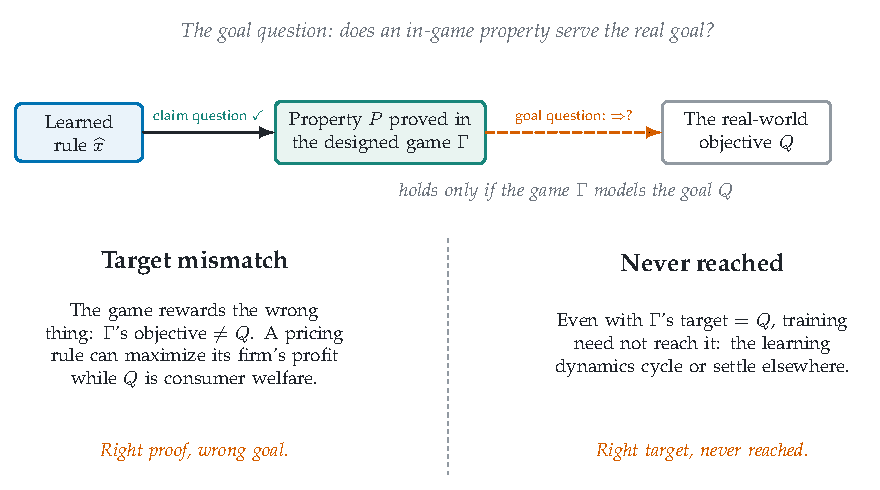
\includegraphics[width=\textwidth]{figure/fig6-goal-question.pdf}
\caption{The goal question. A designed game $\Gamma$ serves the real objective $Q$
only when its target property $P$ supports $Q$ and training reaches a policy with $P$.
The figure highlights two recurring failures: the game's target may fail to support $Q$
(\emph{target mismatch}), as when a pricing rule maximizes its firm's profit while $Q$
is consumer welfare; or the training dynamics may never reach the target even when the
two agree (\emph{never reached}). Both recur in training and oversight and in deployment governance
(\S\ref{sec:gt4ai:governance}); Section~\ref{sec:synthesis} states the same
composition in symbols.}
\label{fig:goal-question}
\end{figure}

\subsubsection{Preference games: what the aggregation certifies}

Preference learning starts from pairwise human comparisons (a person sees two model responses and
says which is better, the data behind RLHF), and must turn many such
comparisons into one policy. How it aggregates them is a design choice that changes the result. Collapsing
each response to a single score discards structure that keeping the
comparisons as a game would preserve. That choice in turn raises two
questions: whether the training converges, and which aggregation it is aiming
at.

Collapsing the comparisons into one hidden score per response, as a Bradley--Terry
model does, forces a straight-line ranking the comparisons need not
have~\citep{BradleyTerry1952}. Three responses can cycle, $A \succ B$, $B \succ C$,
and yet $C \succ A$ --- the rock-paper-scissors pattern again --- as they genuinely do
in psychological, social-choice, and online-comparison
settings~\citep{May1954,Tversky1969,Dudik2015}. A single score cannot represent a
cycle, so an approach built on one loses the cyclic part of the data.

A preference game keeps the comparisons intact and aggregates them through an
equilibrium instead. Nash learning from human feedback (NLHF) takes this route: it reads the
comparison model as a symmetric two-player game and looks for its equilibrium.
It adds one thing, a penalty for drifting too far from the starting policy,
measured in Kullback--Leibler (KL) divergence~\citep{Munos2024}. In plain
terms, the training procedure (Nash-MD) settles on the policy that best answers the
comparisons while staying close to where it began. Because the target rewards staying
near the start, a rival policy can win on the raw comparisons and still lose on the
penalized objective the game actually optimizes.

Whether that training actually reaches the equilibrium is a separate question. Without
such a penalty, in a plain zero-sum
preference game, common update rules can converge only on average while the current policy keeps cycling~\citep{Mertikopoulos2018}: the same
non-transitivity from Section~\ref{sec:gt4ai:evaluation}, now inside training. Building the penalty into the
payoff gives Nash-MD a last-iterate guarantee: in the tabular regularized setting
analyzed by \citet{Munos2024}, the current policy converges at an $O(1/T)$ rate.
Optimistic mirror descent and the extragradient method provide other last-iterate
results under their own game and algorithmic assumptions~\citep{Mertikopoulos2019}.
A convergence claim must specify the game, update rule, and sense of convergence.

Beyond convergence, the methods differ in what they aim at. Some keep this equilibrium
target and only change the optimizer: INPO (iterative Nash policy optimization) folds
no-regret self-play into a single loss, and DNO (direct Nash optimization) uses an
iterative direct-preference update~\citep{Zhang2025INPO,Rosset2024DNO}. Others change the target itself. SPO (self-play preference optimization)
adopts the Minimax Winner from social choice, the response whose worst
pairwise defeat is smallest. It builds cases where the standard reward-based
pipelines, RLHF and direct preference optimization (DPO), fail to recover
it~\citep{Swamy2024SPO}. Its experiments are in continuous control, not LLM
fine-tuning, so that failure is not yet shown for language models. The target is the substantive choice: a Minimax
Winner and a regularized Nash equilibrium turn the same comparisons into different
answers, and no amount of optimization skill decides which answer is the right one.

\subsubsection{Interactive-proof games: what a bounded judge can establish}

The second design depends on a specific asymmetry: a weak judge may be unable to follow
a whole proof yet still able to check one disputed step of it. Debate exploits that gap by
having two provers argue until the dispute narrows to a single step the judge can
actually rule on. Prover--Verifier Games work the same asymmetry from the prover's
side, training the prover to produce reasoning a weaker verifier can check.
Recursive reward modeling, iterated amplification, and process supervision
pursue the same oversight goal through other decompositions. Whether such a game is worth its complexity depends on three things. The
argument must let a limited judge reach conclusions it could not check alone,
it must reward honesty over manipulation, and it must help real judges and not
only idealized ones.

\runin{Formal motivation.} Complexity theory says why an exchange can add power. On its own, a limited judge can
check only claims that come with a short, quickly verifiable certificate: the class \textsc{NP}. Let two provers argue instead, over several back-and-forth rounds, and the
same polynomial-time judge can settle much harder questions. With optimal play
the reachable class is \textsc{Pspace}, the problems solvable with a
polynomial amount of memory, believed to be far larger than
\textsc{NP}~\citep{Irving2018}. The gain comes
from the interaction, not from the judge growing stronger. One subtlety is why debate
uses \emph{two} competing provers rather than one. A single-prover interactive proof lets the verifier run the checks for itself,
which is the \textsc{IP}$=$\textsc{Pspace} result, with \textsc{IP} the class
a randomized polynomial-time verifier can settle. In debate the human judge can
only be consulted as a black box, so the protocol relies instead on a second prover
with an incentive to contest an unsupported step, which leaves the judge to rule
only on a step that has been disputed. These are results about idealized provers and
a formal verifier under optimal play. They motivate the design and bound what such a
protocol could achieve in principle; whether a real judge is more accurate under it
is a separate, empirical question, taken up below.

\runin{Protocol design and assumptions.} The power is not automatic; it depends on who speaks when. \citet{Anil2021} show that if the prover moves first, an optimal prover can
remove all information from its message about the true answer. A protocol
where the verifier commits first restores the guarantees, and a simultaneous
version can settle into the judge simply ignoring the prover. This failure is \emph{information suppression}: the prover withholds the
telling detail rather than overwhelming the judge with evidence.

Even with the right turn order, honesty must be made cheap enough to win.
\citet{Kirchner2024} turn checkability into a training objective, teaching LLM provers
to produce reasoning weaker verifiers can assess, and observe a legibility tax: gains
in checkability can come with lower answer accuracy than correctness-only training. A
sharper problem arises when a wrong argument is easy to state but expensive to
refute~\citep{BarnesChristiano2020}. Doubly-efficient debate bounds the cost on both sides under a restricted
problem model. The honest strategy uses only polynomially more computation
than solving the task, and the verifier makes a fixed number of human-judgment
queries~\citep{BrownCohen2023}, given a human-verifiable record of polynomial
length (with extra conditions in the stochastic case). Prover--estimator
debate targets this information-hiding more directly, giving the honest participant, under
stability assumptions, a strategy about as cheap to run as its
opponent's~\citep{BrownCohen2025ProverEstimator}.

\runin{Evidence with human judges.} Whether any of this helps a real judge is an empirical question.
\citet{Khan2024} vary how strong the debaters are and find that stronger debaters
improve both model and human judges on difficult reading-comprehension questions. The
revealing comparison is with \emph{consultancy}, where a single advocate argues one
side and no one answers back: making that lone advocate more persuasive lowers judge
accuracy, whereas letting two opposed debaters compete raises it. Other studies are less optimistic. \citet{Parrish2022} find single-turn debate-style explanations do not improve
human accuracy in their setting. Across a wider task set, \citet{Kenton2024}
find debate consistently beats that one-sided consultancy, though its
advantage over plain question-answering shows up mainly on
reading-comprehension tasks where the debaters can see a passage the judge
cannot. Across these studies the advantage appears where the judge benefits from
information the interaction reveals and the task admits a useful decomposition; they
do not establish that it holds generally.

Both designs remain limited by what the judge can observe and verify, and both
carry a cost: population methods must train and maintain several
models, and preference self-play and debate add repeated generations and judge
calls. The real question is whether the gain in coverage or checkability is
worth the extra computation. In markets and delegation chains, finally, the interaction is no longer a
training component for one model but an external institution shared by many autonomous
actors.


\subsection{Deployment Governance: From Local Objectives to System Outcomes}
\label{sec:gt4ai:governance}

Once the game is a deployed institution rather than a designed training component ---
the last of the four objects --- no single participant owns the result. Each agent can implement its principal's objective
faithfully, and the system they jointly produce can still be one no principal asked
for. Algorithmic pricing makes this concrete. Even when every pricing agent
maximizes its own firm's profit and adapts well to its rivals, their interaction can
sustain supra-competitive prices and cut consumer surplus, with no individual
principal--agent relationship having failed. The failure is visible only when the
locally successful agents are evaluated together.

Two levers act on such a system, and they act at different moments. Before
deployment, a designer can alter the rules by which agents learn and the information
they see. After deployment, an auditor can test the behavior that actually occurred.
Both have been proposed for pricing. Recent work uses seller data to build
statistical tests of algorithmic pricing and states conditions under which an
algorithm passes~\citep{HartlineLongZhang2024,HartlineWangZhang2025}, while
\citet{Harrington2018} separately proposes making collusion by autonomous pricing
agents unlawful. In each case, the audit or the legal standard fixes the
alternatives a seller is compared against and the burden of proof it carries. That
choice, in turn, dictates what data must be collected.

The rest follows the dependencies among these choices. The objective and the affected
parties come first, because they fix what would count as a failure: in pricing,
consumers sit outside every principal--agent pair and still absorb the harm. The
objective then constrains the two levers, how the algorithm updates, fixed before
deployment, and which deviations an audit tests, applied after it. The lever chosen
fixes what the audit record must contain, down to the randomization a seller must
log. And the record fixes the scope of the inference it supports, from one seller's
conduct to a claim about the market.

\subsubsection{System objective and affected parties}
Naming the objective is harder than it sounds, because the natural accounting leaves
parties out. A local equilibrium or regret guarantee states a property that holds
inside the interaction as specified. Extending it to a claim about the system takes a
separate argument: who is affected, and what the institution is for. Delegation
games place that gap inside the principal--agent relation. \citet{Sourbut2024} separate two ways this can go wrong. A control failure is an
agent not doing what its principal wanted. A cooperation failure is agents interacting
badly even though each serves its own principal well. Both decompose into alignment and
capability components, with principal welfare as the evaluative object. Because principal welfare depends on collective
cooperation as well as on individual control, a property proved for one
principal--agent pair says nothing about the collective half.

Pricing adds a party the accounting misses entirely. Consumers are not principals in
the delegation game, so no term in it tracks what happens to them. Coordination among
profit-aligned pricing agents can therefore be a cooperation success by that measure
and a system failure the moment consumer welfare enters the objective. Deciding whose
outcomes count is thus a prior step rather than a detail of implementation: it fixes
which of those two readings the same behavior receives.

\subsubsection{Ex ante design of learning and information}
With the objective fixed, the earlier lever chooses how the agent learns and what it
is allowed to see. The algorithmic-pricing literature shows how much rides on that
choice. \citet{Calvano2020} find that Q-learning agents in repeated Bertrand
competition with differentiated products learn supra-competitive prices without any
direct communication. The learned strategies show punishment phases followed by a return to high prices, though the analysis proves no general
convergence theorem for Q-learning. \citet{Asker2022} isolate one source of this sensitivity: how the
algorithm updates. With no weight on future profits, synchronous updating, which computes returns for every price and not just the
one chosen, yields competitive prices in their baseline, whereas asynchronous updating can push prices near the
monopoly level. Once future profits carry positive weight, even synchronous updating
permits supra-competitive prices, though still less than asynchronous.
\citet{BanchioSkrzypacz2022} find the same sensitivity in what agents are told rather
than in how they update. In a repeated auction with two bidders of equal normalized
value and a discrete bid grid, first-price auctions sustain bids below the competitive
benchmark when bidders receive no extra feedback; revealing the lowest winning bid
raises competitiveness.

Theory and field evidence bear on the same sensitivity. \citet{Cartea2025} prove a
Folk-theorem-style result for boundedly rational learners using finite-memory
strategies in repeated potential games, a restricted class that does not transfer
directly to general differentiated Bertrand competition.
\citet{FishGonczarowskiShorrer2024} study LLM agents in place of hand-built learners:
their oligopoly experiments reach supra-competitive prices quickly and autonomously,
and seemingly innocuous changes to the prompt alter how far prices rise.
\citet{Assad2024} supply field evidence from German retail gasoline markets that are
not monopolies. Using headquarters-level adoption as an instrument, they estimate that
algorithmic pricing raises margins, with margins rising in duopoly and triopoly
markets once all competing stations adopt. The lesson for governance is direct: the
``algorithm'' label alone does not fix the market behavior to be evaluated. The update
rule and the information feed are what an ex ante standard would have to specify, and
an audit after the fact tests something different, namely whether the behavior
a deployment actually produced meets a standard.

\subsubsection{Ex post standards and deviation classes}
An audit tests behavior against alternatives the auditor names, so a standard is only
as strong as the set of alternatives behind it. That set is the deviation class. The choice among
classes settles three things in turn: what a passing seller has actually ruled out,
what a market of passing sellers collectively satisfies, and whether an algorithm can
pass the test while still doing harm.

The classes differ in how much a hypothetical deviator is allowed to change. External
regret compares realized profit against what one fixed price, used in every round,
would have earned. Internal regret asks a narrower question: would replacing one
chosen action $i$ by another $j$ have paid? Swap regret allows a separate replacement
for every chosen action. Calibrated regret is the version of swap regret written for
posted prices. For a finite price set $\mathcal{P}$, it is the largest average gain
available from any remapping $\sigma:\mathcal{P}\rightarrow\mathcal{P}$ that replaces
each posted price $p$ by $\sigma(p)$, holding that round's demand environment
fixed~\citep{HartlineLongZhang2024}. A seller with low calibrated regret has therefore
ruled out every profitable price-contingent remapping, a strictly finer test than
fixed-price deviations.

Passing that test everywhere supports a market-level statement, but a limited one. When
every player has vanishing internal regret, the empirical distribution of joint
actions approaches the set of correlated equilibria of the stage
game~\citep{FosterVohra1997,HartMasColell2000,BlumMansour2007}. That theorem
constrains conditional incentives in the observed distribution and nothing else. It
carries no welfare criterion and no legal one, so calling the resulting distribution
``competitive'' takes a benchmark the theorem does not supply.

\citet{HartlineLongZhang2024} supply one, defining unilateral non-collusion through
calibrated best response: conditional on whatever a seller's own price reveals, that
price must approximately maximize its expected profit in the demand environment that
price induces. The conditioning is essential, because the pattern of posted prices can
itself be information a seller acts on. Low calibrated regret is the dynamic version
of this condition, measured over a deployment history, and when every seller meets it
the joint price distribution forms a correlated equilibrium of the stage pricing game.
\citet{Hartline2026} then designates stage-game equilibrium prices as competitive and
the additional repeated-game equilibria as non-competitive. That gives the deviation
condition a concrete, usable meaning, while leaving the market assumptions and the welfare or legal benchmark as separate inputs. The correlated-equilibrium
result itself still implies nothing about consumer surplus.

Changing the deviation class changes which harmful behaviors can pass the test.
\citet{Braverman2018} exhibit a seller facing a buyer who runs EXP3, or any other
algorithm that responds to average past payoffs, and show the seller can extract
nearly the buyer's full welfare. The same paper builds a different no-regret algorithm
for the buyer, against which the seller can do no better than repeatedly posting the
Myerson reserve. Both buyer algorithms are no-regret by the same external standard;
the losses they expose the buyer to differ sharply.
\citet{HartlineWangZhang2025} make a matching point on the seller side, showing that
algorithms satisfying only best-in-hindsight regret can be driven to post
supra-competitive prices even when neither seller has side information.

External regret misses all of this because it compares the whole realized sequence
against a single fixed action. A profitable deviation can be conditional instead ---
replace price $p$ by $q$, but only in the rounds where $p$ was posted --- with no
single fixed price improving the average. Calibrated regret tests exactly those
price-contingent replacements, and a seller can satisfy it on its own, whatever its
rivals do.

\subsubsection{Auditability from deployment records}
Having the right test is not the same as being able to run it. Calibrated regret asks
what a seller would have earned at prices it did not post, and no record contains that
directly. \citet{HartlineLongZhang2024} recover it from a deployment log that keeps
three things per round: the price posted, the demand realized at that price, and the
distribution the seller drew that price from. Because the seller sometimes prices at
random, rarely posted prices still appear in the log, and demand at them can be
estimated by weighting the observed rounds by how likely each price was: the
inverse-propensity construction. The rarer a price, the more rounds it takes
to identify, so the data requirement grows as the smallest probability the algorithm assigns
to any price shrinks.

That gives a seller something to act on: deliberately adding exploration and logging
makes a competitive deployment auditable. The estimator needs no access to source
code, only credible internal records of the randomization and the outcomes, a logged
black-box audit whose validity rests entirely on the provenance and integrity
of the transcript.

An incomplete record yields a bound rather than a verdict. Pessimistic calibrated
regret drops the requirement that every price be posted with positive
probability~\citep{HartlineWangZhang2025}: where the transcript leaves a
counterfactual outcome unidentified, it reports the highest calibrated regret
consistent with any completion of the missing data. A low pessimistic value certifies
low regret under every compatible completion. A high value is ambiguous by construction: it may signal a real profitable
deviation, or only a record too thin to rule one out. The authors read a failure to supply a
low-regret certificate as violating a proposed per se rule, which places the
evidentiary burden on the seller. That is a legal choice, not a statistical one.

Unknown costs draw a second boundary of a different kind. Regret is computed from
profit, profit requires marginal cost, and the auditor rarely knows it. Suppose the auditor
lets marginal cost lie anywhere in a set $\mathcal{C}$. A seller then passes the
plausible-non-collusion test as soon as some $c\in\mathcal{C}$ makes its observed
behavior look low-regret, even when the true cost would imply high regret. A high
assumed cost can thus rationalize supra-competitive prices that were in fact generated
at a lower one, and the wider $\mathcal{C}$ is, the weaker the test becomes. How wide
it may be is set by the cost evidence available and by the governing legal standard,
not by the data alone.

\subsubsection{From individual evidence to market-level conclusions}
A clean audit of one seller remains a statement about that seller. Getting from there
to a claim about the market is not automatic, and the gap has been made explicit.
\citet{Arunachaleswaran2025} study sequential deployment: the first seller commits to
any no-regret algorithm, and the second then optimizes against the environment that
commitment creates. Supra-competitive prices arise whenever the second seller earns at least what random pricing would earn, including when its choices are
restricted to price distributions that ignore what the first seller does. They also construct an
equilibrium in algorithm space with near-monopoly prices and no threats written into
either algorithm. \citet{HartlineClarification2026} classifies that outcome as
non-competitive while declining to call it collusion. One seller learns a best
response; the other uses the non-competitive static strategy. The outcome violates the
stage-game competitive benchmark, yet the evidence is not enough to show that the two
acted jointly.

The lesson is about scope. Low calibrated regret is a property of an individual
seller; the correlated-equilibrium conclusion is a property of the market, and it
follows only when \emph{every} seller has it. Let one seller fail and the market-level
conclusion is gone. Whether antitrust law should prohibit high-regret or naively
non-optimizing pricing when no agreement is proven is a policy question, and a failed
audit by itself does not establish an agreement among
sellers~\citep{Harrington2018}.

The two levers, then, act at different times and answer different questions. Design
before deployment changes the update rule or the information structure; auditing after
it evaluates the behavior that resulted. When every seller has low calibrated regret,
the data do impose a stage-game equilibrium restriction on the market outcome. That
restriction answers the claim question and leaves the goal question open: whether the
market it describes is one a regulator should accept. Answering it takes an explicit objective for each
agent and a separate criterion for the market. A seller can optimize the objective it
was assigned even when the market it helps produce fails the criterion that matters.
